%%%%%%%%%%%%%%%%%%%%%%%%%%%%%%%%%%%%%%%%%
% Simple Sectioned Essay Template
% LaTeX Template
%
% This template has been downloaded from:
% http://www.latextemplates.com
%
% Note:
% The \lipsum[#] commands throughout this template generate dummy text
% to fill the template out. These commands should all be removed when 
% writing essay content.
%
%%%%%%%%%%%%%%%%%%%%%%%%%%%%%%%%%%%%%%%%%

%----------------------------------------------------------------------------------------
%	PACKAGES AND OTHER DOCUMENT CONFIGURATIONS
%----------------------------------------------------------------------------------------

\documentclass[12pt]{article} % Default font size is 12pt, it can be changed here

\usepackage{geometry} % Required to change the page size to A4
\geometry{a4paper} % Set the page size to be A4 as opposed to the default US Letter

\usepackage{graphicx} % Required for including pictures
\graphicspath{{Images/}}



\usepackage{float} % Allows putting an [H] in \begin{figure} to specify the exact location of the figure

\linespread{1.2} % Line spacing

%\setlength\parindent{0pt} % Uncomment to remove all indentation from paragraphs

%\graphicspath{{Images/}} % Specifies the directory where pictures are stored


\newcommand{\job}{\texttt{Asp::Job}}
\newcommand{\model}{\texttt{Asp::Model}}
\newcommand{\solver}{\texttt{Asp::Solver}}
\newcommand{\configuration}{\texttt{Asp::Configuration}}
\newcommand{\constraint}{\texttt{Asp::Constraint}}
\newcommand{\entry}{\texttt{Timetable::Entry}}
\newcommand{\run}{\texttt{run()}}

\begin{document}

%----------------------------------------------------------------------------------------
%	TITLE PAGE
%----------------------------------------------------------------------------------------

\begin{titlepage}

\newcommand{\HRule}{\rule{\linewidth}{0.5mm}} % Defines a new command for the horizontal lines, change thickness here

\center % Center everything on the page

\textsc{\LARGE University of Potsdam}\\[1.5cm] % Name of your university/college
\textsc{\Large Declarative Modeling}\\[0.5cm] % Major heading such as course name
%\textsc{\large Timetabling Project}\\[0.5cm] % Minor heading such as course title

\HRule \\[0.4cm]
{ \huge \bfseries Timetabling Project}\\[0.4cm] % Title of your document
\HRule \\[1.5cm]

\begin{minipage}{0.4\textwidth}
\begin{flushleft} \large
\emph{Author:}\\
  Robert Sch\"afer \\
  Felix Kubicek
\end{flushleft}
\end{minipage}
~
\begin{minipage}{0.4\textwidth}
\begin{flushright} \large
\emph{Supervisor:} \\
  Javier Romero Davila
\end{flushright}
\end{minipage}\\[4cm]

{\large \today}\\[3cm] % Date, change the \today to a set date if you want to be precise


%\includegraphics{Logo}\\[1cm] % Include a department/university logo - this will require the graphicx package

\vfill % Fill the rest of the page with whitespace

\end{titlepage}

%----------------------------------------------------------------------------------------
%	TABLE OF CONTENTS
%----------------------------------------------------------------------------------------

\tableofcontents % Include a table of contents

\newpage % Begins the essay on a new page instead of on the same page as the table of contents 

%----------------------------------------------------------------------------------------
%	INTRODUCTION
%----------------------------------------------------------------------------------------

\section{Introduction} 

Our goals in this project have been to satisfy our customer and to train ourselves in project management.
We therefore carried out a considerable amount of requirements engineering.
Also we decided to work under agile development principles.
We developed a rapid prototype and continued on delivering a new version of our software each iteration.
Besides that we ensured that we keep each change or new feature covered by unit and integration testing.
Our code is hosted online on Github as open source and we accomplish a good knowledge transfer among the team by using pull requests.



\section{Architecture} % Sub-section

We give an overview by showing two parts of our architecture.

\subsection{Data Model} 

\begin{figure}[h]
    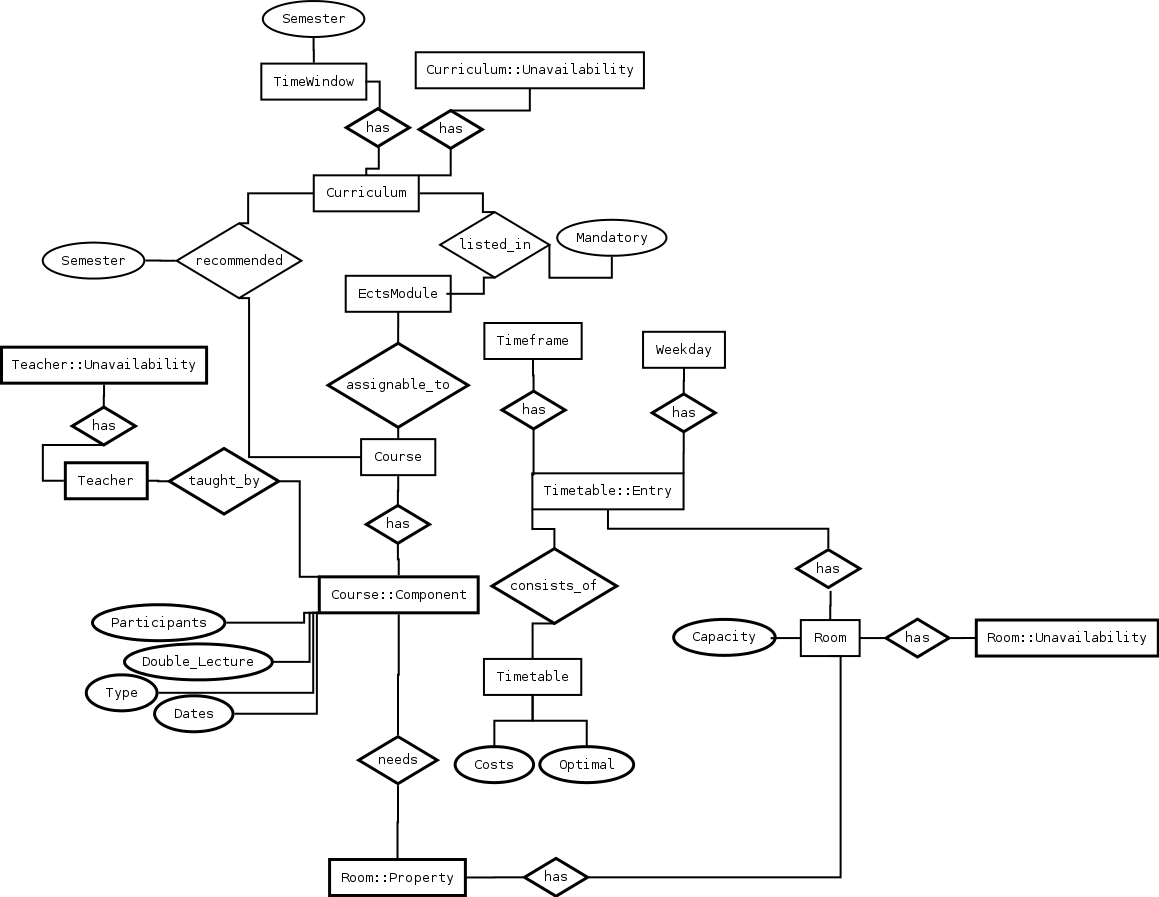
\includegraphics[width=\textwidth]{TimetablingER_Dia.png}
    \label{fig:schema}
\end{figure}

Figure~\ref{fig:schema} demonstrates the database schema.
A timetable, which consists of several timetable entries, represents a complete schedule.
Timetables have costs, resulting from penalty values of the ASP soft constraints.
The timetables with the lowest costs are optimal solutions.
A timetable entry is an assignment of a certain component of a course, e.g. a lecture, to a certain room, as well as to a specific weekday and timeframe. 
Course Components, taught by a specific teacher, have got a certain type, e.g lecture, tutorial, etc.
Besides course components can have multiple dates, participants and several room properties.
If, for instance, the course component has to take place in a computer pool then the room assigned to the course component has to be declared as computer pool through a certain property.
The courses are linked to a specific curriculum through modules.
Besides a course can be recommended for a semester in a certain curriculum.
The advantage over recommending modules for a specific semester is that courses with different recommendations can now be assigned to the same module.
The modules listed in a specific curriculum can be elective or mandatory.
A curriculum can be assigned to multiple time windows.
The concept of time windows was introduced to allow students participating the \emph{Informatik Lehramt Bachelor} program to study with little overlapping of courses.
In order to prevent overlapping, mandatory lectures for student teachers has to be assigned to a determined set of time windows dependent on the semester recommendation.

Finally there are unavailabilities for teachers, curriculum and rooms.
All unavailabilities are linked to a specific day and time-slot which is not shown in the diagram for clarity reasons.

\subsection{ASP Integration} 

\begin{figure}[h]
    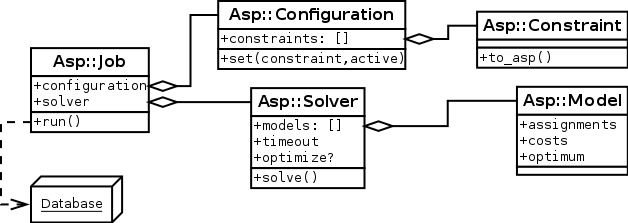
\includegraphics[width=\textwidth]{Images/AspClassDiagram.png}
    \label{fig:class_diagram}
\end{figure}

Figure~\ref{fig:class_diagram} demonstrates the integration of the answer set solving.
In the final encoding we have facts and rules.
A fact corresponds to an entity in the database and a rule corresponds to an \constraint{}.
In order to get all the necessary information from the database to create the desired asp encoding we use the \job{} class.
The main method in this tool chain is the \run{} method.
All entities which are required for the encoding are transformed into facts.
The \job{} then receives a set of constraints from the configuration.
The configuration can enable or disable a certain \constraint{} and in the future it will be used to change the weight of each \constraint{}.
The information is then put together and send to the \solver{} which receives an encoded asp problem as text.
The \solver{} provides the interface to the user's shell and is also responsible to create a \model{} for each found solution.
These \model{} classes are used to parse ruby objects from the strings which are returned by clasp.
So to give an example, every \entry{} is parsed from the answer set.
Also, we parse a violation of a soft constraint from the answer set, associated with the conflicting objects.
Note that violations have to be parsed at the end for this reason.
They are associated to entries of the same answer set which have to be present at the time.
Subsequent to the parsing, the job class then saves all the generated objects in the database.
The state in the database is then used as the input for the visualization of the timetable.


\section{Conclusion}


%----------------------------------------------------------------------------------------
%	BIBLIOGRAPHY
%----------------------------------------------------------------------------------------

\begin{thebibliography}{99} % Bibliography - this is intentionally simple in this template

%\bibitem[Figueredo and Wolf, 2009]{Figueredo:2009dg}
%Figueredo, A.~J. and Wolf, P. S.~A. (2009).
%\newblock Assortative pairing and life history strategy - a cross-cultural
%  study.
%\newblock {\em Human Nature}, 20:317--330.
 
\end{thebibliography}

%----------------------------------------------------------------------------------------

\end{document}
